\documentclass[]{article}
\usepackage{amsmath}
\usepackage{amssymb}
\usepackage{stmaryrd}
\usepackage{latexsym}
\usepackage{graphicx}
\usepackage{fancyhdr}
\usepackage{color}
\usepackage{listings}
\usepackage[top=1in, right=0.75in, left=0.75in]{geometry}
\usepackage[colorlinks=true, linkcolor=blue]{hyperref}

\definecolor{customgreen}{rgb}{0,0.6,0}
\definecolor{customgray}{rgb}{0.5,0.5,0.5}
\definecolor{custommauve}{rgb}{0.6,0,0.8}

\definecolor{dkgreen}{rgb}{0,0.6,0}
\definecolor{gray}{rgb}{0.5,0.5,0.5}
\definecolor{mauve}{rgb}{0.58,0,0.82}

\lstset{frame=tb,
	language=MATLAB,
	aboveskip=3mm,
	belowskip=3mm,
	showstringspaces=false,
	columns=flexible,
	frame=single,	                   % adds a frame around the code
	basicstyle={\small\ttfamily},
	numbers=none,
	numberstyle=\tiny\color{gray},
	keywordstyle=\color{blue},
	commentstyle=\color{dkgreen},
	stringstyle=\color{mauve},
	breaklines=true,
	rulecolor=\color{black},
	breakatwhitespace=true,
	tabsize=3,
	numbers=left,                    % where to put the line-numbers; possible values are (none, left, right)
	numbersep=10pt,                   % how far the line-numbers are from the code
	numberstyle=\tiny\color{customgray}, % the style that is used for the line-numbers
}

\author{
	Mohammad Hossein Shafizadegan\\
	99104781
}
\title{
	Coding Assignment 1 \\
	Computational Intelligence  \\
	Dr. S. Hajipour
}

\pagestyle{fancy}
\rhead{CI}
\lhead{CHW 1}

\newcommand{\pict}[2]{\begin{center}
		\includegraphics[width=#1\linewidth]{Fig/#2.png}
\end{center}}
\newcommand{\mat}[1]{\begin{bmatrix} #1 \end{bmatrix}}
\newcommand{\deter}[1]{\begin{vmatrix} #1 \end{vmatrix}}

\definecolor{customgreen}{rgb}{0,0.6,0}
\definecolor{customgray}{rgb}{0.5,0.5,0.5}
\definecolor{custommauve}{rgb}{0.6,0,0.8}

\definecolor{dkgreen}{rgb}{0,0.6,0}
\definecolor{gray}{rgb}{0.5,0.5,0.5}
\definecolor{mauve}{rgb}{0.58,0,0.82}

\lstset{frame=tb,
	language=MATLAB,
	aboveskip=3mm,
	belowskip=3mm,
	showstringspaces=false,
	columns=flexible,
	frame=single,	                   % adds a frame around the code
	basicstyle={\small\ttfamily},
	numbers=none,
	numberstyle=\tiny\color{gray},
	keywordstyle=\color{blue},
	commentstyle=\color{dkgreen},
	stringstyle=\color{mauve},
	breaklines=true,
	rulecolor=\color{black},
	breakatwhitespace=true,
	tabsize=3,
	numbers=left,                    % where to put the line-numbers; possible values are (none, left, right)
	numbersep=10pt,                   % how far the line-numbers are from the code
	numberstyle=\tiny\color{customgray}, % the style that is used for the line-numbers
}

\begin{document}
	\begin{figure}
		
\includegraphics[width=0.25\textwidth]{Fig/Sharif.png}
		\centering
	\end{figure}
	\maketitle
	\tableofcontents
	\newpage
		%-----------------------------------------------------------------------------------------------------------------	
	\section{Question 1}
	\subsection*{a}
	In order to obey clean code rules, we have a developed a function called "plot\_fact" for this section. The initial values of the parameters will be provided to this function as input arguments.
	\begin{lstlisting}
		function plot_fact(init_w1, init_w2, init_T, beta)
	\end{lstlisting}
	 In this function, we have to define and create a \textit{meshgrid} for $X$ and $Y$ as follows:
	\begin{lstlisting}
		global p % define a global variable for the plot handle
		dx = 0.01;
		dy = 0.01;
		beta = 0.5;
		
		x = -1:dx:1;
		y = -1:dy:1;
		[X,Y] = meshgrid(x,y);
	\end{lstlisting}
	Then we assign random initial values to $w_1$, $w_2$, and $T$ and form the activation function.
	\begin{lstlisting}
		% initialize some initial values for w1, w2, and T
		w1 = 0.5;
		w2 = 0.5;
		T = 0.5;
		
		f_act = 1./(1 + exp(-1*beta.*(w1*X+w2*Y-T))); % calculate the initial f_act values
	\end{lstlisting}
	After that we have to deal with interactive sliders for each of the parameters. Using MATLAB builtin \textit{uicontrol} command, we create three sliders. The code used for creating one of these sliders can be seen below.
	\begin{lstlisting}
		% Slide bar for w1
		s_w1 = uicontrol('Parent',f,'Style','slider','Position',[81,110,419,23],...
									   'value',w1, 'min',-5, 'max',5);
		bgcolor = f.Color;
		sl1 = uicontrol('Parent',f,'Style','text','Position',[50,110,23,23],...
								   'String','-5','BackgroundColor',bgcolor);
		sl2 = uicontrol('Parent',f,'Style','text','Position',[500,110,23,23],...
								   'String','5','BackgroundColor',bgcolor);
		sl3 = uicontrol('Parent',f,'Style','text','Position',[240,85,100,23],...
								   'String','w1','BackgroundColor',bgcolor);
	\end{lstlisting}
	In order to interactively change the parameters and observe the results, we have to develop a callback function for the sliders and assign the callback function to them. In the callback function, we first parse the new value of the parameters, then we generate the activation function again regarding new values. The code for the callback function is as follows:
	\begin{lstlisting}
		function update (src, event, b_w1, b_w2, b_T)
			global p % access the global variable p
			dx = 0.01;
			dy = 0.01;
			beta = 0.5;
			
			x = -1:dx:1;
			y = -1:dy:1;
			[X,Y] = meshgrid(x,y);
			
			w1 = get(b_w1, 'Value'); % get the current slider value for w1 using the get function
			w2 = get(b_w2, 'Value'); % get the current slider value for w2 using the get function
			T = get(b_T, 'Value'); % get the current slider value for T using the get function
			f_act = 1./(1 + exp(-1*beta.*(w1*X+w2*Y-T))); % calculate the new f_act values
			p.ZData = f_act; % update the plot 
			
			fprintf("w1= %d   ,   w2 = %d   ,   T = %d \n", w1, w2, T);
			
		end
	\end{lstlisting}
	The result can be seen below:
	\pict{0.5}{Q1_F1}
	
	\subsection*{b}
	Here we simply set $w_1=w_2=T=\beta=1$. The results will be as follows:
	\begin{center}
		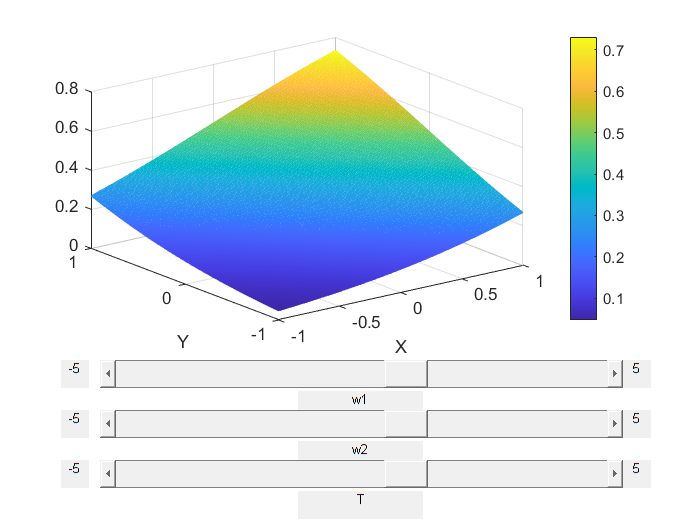
\includegraphics[width=0.4\linewidth]{Fig/Q1_F2.png}
		\qquad\qquad
		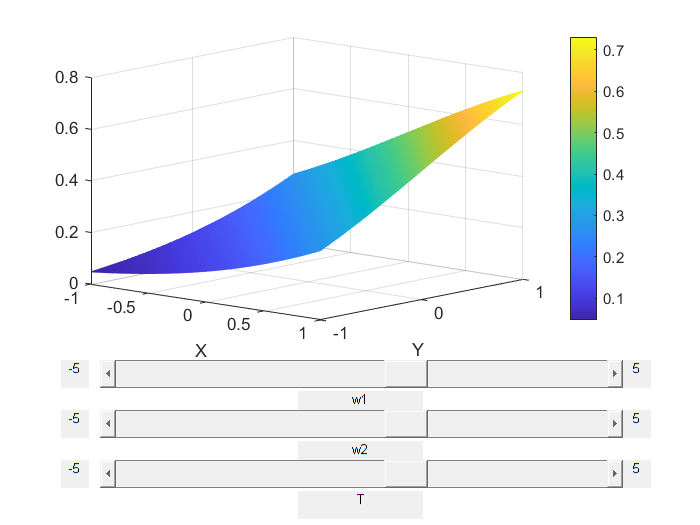
\includegraphics[width=0.4\linewidth]{Fig/Q1_F3.png}
	\end{center}

	\subsection*{c}
	In order to implement the OR function, we have to set the value of each weights equal to 2 and the threshold will be 1. As it is said in the instructions, we choose a huge value for $\beta$, e.g. 100.
	\begin{lstlisting}
		%% part C
		
		% OR function
		w1 = 2;
		w2 = 2;
		T = 1;
		
		beta = 100;
		
		plot_fact(w1, w2, T, beta)
	\end{lstlisting}
	The results can be seen here.
	\begin{center}
		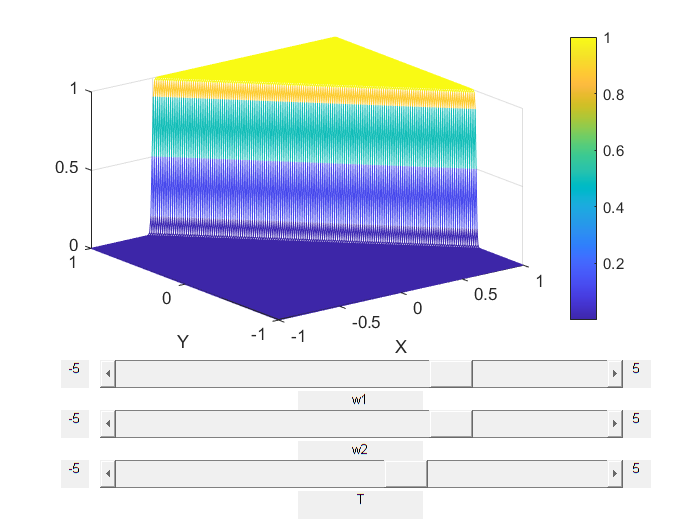
\includegraphics[width=0.4\linewidth]{Fig/Q1_F4.png}
		\qquad\qquad
		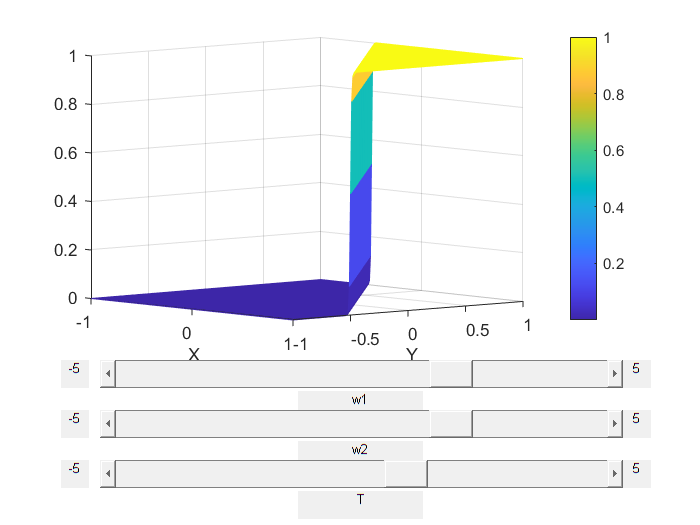
\includegraphics[width=0.4\linewidth]{Fig/Q1_F5.png}
	\end{center}
	Based on the above figures, it can be concluded that the activation function for huge values of $\beta$ is quite the same as step threshold function.
	
	\subsection*{d}
	Now we set the value of $\beta$ to 0.1 and visualize the results.
	\pict{0.5}{Q1_F6}
	
\end{document}